\chapter{Related work}\label{ch:related-work}
%
% =========================
%      old introduction
% =========================
% \section{Introduction}\label{introduction}
% Fairness in Machine Learning is a topic that has recently received increasing attention.
% Machine Learning has become very widespread in our society
% which brings some dangers with it.
% Decisions such as credit eligibility and hiring are increasingly done automatically.
% However, the algorithms that are used in these decisions can have strong biases
% that stem from the training data.
% Often, the algorithms are even more biased than the training data.
% \citet{kamishima2012fairness} give a great illustration for this
% (adapted from \citet{calders2010three}).
% The illustration is based on the Adult/Census Income dataset \citep{kohavi1996scaling}
% which contains records of individuals with thirteen attributes, among them age and gender.
% The task is to predict whether or not the individual earns more than \$50K per year.
% In the dataset, 32\% of the men have a positive label (\ie, they earn more than \$50K),
% but of the women only 11\% have a positive label.
% With this ratio of about 3:1, the dataset is already skewed.
% However, when training a \href{https://en.wikipedia.org/wiki/Naive_Bayes_classifier}{Na\"ive Bayes classifier} on the data,
% the ratio in the predictions is even more unfair:
% the amount of women who get a positive prediction is even lower than 11\%.
% If the Na\"ive Bayes classifier does not get access to the gender information,
% the predictions will be a bit fairer,
% but they are still more unfair than the original dataset labels.
%
% This phenomenon of predictions being more unfair than an already skewed dataset
% is due to the generalisation that classifiers have to make.
% It is easier to classify all but the most outstanding women as low income
% than to learn a complicated decision boundary.
% Furthermore, removing the gender information does not solve the problem
% because the gender can be inferred from other data.
%
% The following is a review of the literature on Fairness in Machine Learning.
% Several different approaches to and definition of Fairness are presented.
% The focus is on identifying the major trends in the field from the beginning.
%
\begin{figure}[tbp]
  \resizebox{\textwidth}{!}{
    \begin{forest}
    forked edges,
    for tree={rounded corners, edge+={darkgray, line width=1pt}, draw=darkgray, align=center, anchor=children},
    before packing={where n children=3{calign child=2, calign=child edge}{}},
    before typesetting nodes={where content={}{coordinate}{}},
    where level<=1{line width=2pt}{line width=1pt},
    [methods for algorithmic fairness
      [data de-biasing, line width = 2pt
        [dropping\\features]
        [additional\\synthetic data]
        [
          [fair representations
            [non-parametric
              [HSIC]
              [MMD]
            ]
            [adversarial networks
              [sample-wise, draw=blue]
              [set-wise, draw=blue]
            ]
          ]
        ]
      ]
      [post-hoc methods, line width = 2pt
        [separate\\models]
        [threshold\\shifting]
      ]
      [
      [change to train-\\ing procedure, line width = 2pt
        [modified sampling]
        [
          [change to loss
            [
              [change of optim-\\isation target, draw=blue]
              [constrained\\optimisation]
            ]
          ]
        ]
        [loss reweighting]
      ]]
    ]
    \end{forest}
  }
  \caption{%
    Taxonomy of fairness methods.
    The three categories with blue borders correspond to those categories
    under which the proposed models in this thesis fall (see \chapref{ch:content} for details).
    This diagram does not show all the axes along which methods can vary.
    In particular, it does not distinguish between different intended \emph{settings}.
  }%
  \label{fig:fairness-taxonomy}
\end{figure}%
%
\section{Two views of the dataset bias problem}\label{two-views-of-the-dataset-bias-problem}
As alluded to in the introduction,
there is a divide in the relevant literature in how the problem of dataset bias is approached.
On the one hand, there is the ``ground-truth-centric'' view -- expressed through most of the introduction --
that the training set is biased but the deployment setting is not.
By \emph{deployment setting} I am here referring to the real distribution
that will be encountered by the machine learning system once it is in use.

% This can be seen as a form of transfer learning and notably does not exhibit a fairness-accuracy trade-off.

An instance of this setting has been formalised by \citet{blum2020recovering}.
In their formalisation, the training set starts out unbiased,
but then, for samples with \(s=0\), class labels \(y\) are flipped from 1 to 0 with probability \(\nu\).
In addition, samples with \(s=0\) and \(y=0\) are dropped with probability \(1-\beta_\mathit{NEG}\)
and those with \(s=0\) and \(y=1\) are dropped with probability \(1-\beta_\mathit{POS}\).
Meanwhile, the test remains unbiased and is the basis for evaluating our models.

On the other hand, there is the ``definition-centric'' view that,
given some training data and not necessarily knowing anything about the deployment setting,
we define \emph{fairness criteria} which a fair classifier should satisfy.
Here, the primary goal is not to correct for the deviation of the training data from the true distribution,
but simply to ensure that the classifier is fair in some specific sense.
By default, a classifier would \emph{not} be fair in that specific way.
It is left open as to whether this unfairness originates from the training data or from the algorithm itself.
Evaluation is typically performed on a test set that has all the same biases as the training set,
and thus gives rise to a fairness-accuracy trade-off.

The first works in the field almost exclusively took the definition-centric view,
most of them using \acf{DP} \citep{dwork2012fairness} as the fairness criterion.

The boundary between these views is not completely clear-cut.
Consider the case where a biased training set is available,
and an unbiased test set is assumed to exist, but we do not have access to it \citep{jiang2020identifying}.
Then we might at least know that the unbiased test set satisfies \ac{DP}.
In this case, testing the classifier for \ac{DP} is an indication
for how well it would fare on the unbiased test set.

Furthermore, there is significant overlap in the solutions employed for the two views:
a method developed for one of them can often be adapted to the other as well.

The works discussed in the beginning of this chapter are mostly taking the definition-centric view.
Towards the end, I discuss more works with the other viewpoint.

\Figref{fig:fairness-taxonomy} provides a high-level overview
of one possible categorisation of the methods presented here.
It can serve as a map for navigating through this chapter.
% It is meant as a rough guide through the chapter.

\section{Foundations of algorithmic fairness}\label{sec:foundations}
This section discusses the publications that lay the ground work for the algorithmic fairness literature.
More recent publications are discussed in %
\secref{sec:refinement-on-previous-ideas-for-fair-classification-and-fair-representations}.

\subsection{Precursors}\label{precursor}
The first published work to address the problem of biases in machine learning
was arguably the work by \citet{pedreshi2008discrimination}
with the main focus being data-mining.
Their first fundamental conclusion
is that it is not sufficient to remove the protected attribute
(which should not be used as a basis for prediction) from the data.
That is, if the information about, for example, race
is removed from the data,
there is usually enough background information to reconstruct that attribute.
In their context of data mining,
they distinguish between direct and indirect discrimination:
the former explicitly uses discriminatory features in the premise of the rule,
while the latter uses features that are closely associated with discriminatory features%
\footnote{This is similar to the legal view of direct and indirect discrimination
where direct discrimination is when people with a specific protected characteristic are treated worse,
whereas indirect discrimination is a policy that does not make direct references to a protected characteristic
but disproportionally affects people with a specific characteristic.}.
% The latter case can be
% detected by checking the other rules in the dataset.

\subsection{Modification of labels for fairness enforcement}%
\label{modification-of-labels-for-fairness-enforcement}
Independently of \citet{pedreshi2008discrimination}, but with a similar intention,
\citet{kamiran2009classifying} considered discrimination in classification tasks.
Their goal is to modify the dataset so that any classifier trained on it will be ``fair'';
a condition which is measured with a fairness metric on the test set predictions.
The test set is drawn from the same distribution as the training set.
To demonstrate their method, they use the ``German credit dataset''~\citep{Dua:2017}
where the task is to classify people as a good or a bad credit risk.

The authors formulate the problem as it was later done in other works on fairness:
there is a set of features \(x\), a binary class label \(y\)
and a special \emph{sensitive attribute} \(s\) which determines the demographic group.
The sensitive attribute \(s\) is assumed to be binary in the derivation,
but does not have to be.
\(s=0\) refers to the group vulnerable to discrimination and \(s=1\) to all other individuals.
It is further assumed that one of the class labels is generally desirable;
for example, it might correspond to being accepted for a loan or being given bail.
This class label is referred to as the positive label: \(y = 1\).

The authors then define a concrete measure of discrimination (where $\hat{y}$ refers to the prediction of a classifier):
\begin{align}
  \label{eq:disc}
  Disc := P(\hat{y}=1|s =1) - P(\hat{y}=1|s = 0)~.
\end{align}
% (The paper uses a different notation.
% The notation here reflects the notation in later papers.)
It is zero when the individuals in both groups have the same chance to get a positive prediction.
Thus, it measures the violation of \ac{DP}, where $Disc=0$ corresponds to satisfying \ac{DP}.

Their algorithm for de-biasing the dataset comprises two steps.
First, a well-calibrated classifier (Na\"ive Bayes in the paper) is trained on the data
\emph{without} the sensitive attribute.
This classifier is then used to determine a ranking for how likely a positive label is for a given individual.
The highest ranked individuals that have label \(y=0\)
and are potentially discriminated against (\(s=0\)) get ``promoted'' to \(y=1\)
and the lowest ranked individuals with label \(y=1\) and \(s=1\) get ``demoted'' to \(y=0\)
until the dataset is fair according to the \(Disc\) measure.
The idea being that the ranking ensures that the changes in the dataset
happen to the most appropriate candidates (those closest to the decision boundary);
the main goal being a prevention of a big drop in accuracy of the final classifier
on the test set whose distribution matches the training set.

% The paper concludes with results on the German credit data,
% using Na\"ive Bayes for ranking and also for the final classifier.
% Using \emph{Age} as the sensitive attribute,
% the dataset itself shows a \(Disc\) of about 15\% (depending on the train-test split).
% As a baseline, a Na\"ive Bayes classifier was trained with the sensitive attribute
% resulting in \(Disc = 25\%\).
% Without the sensitive attribute it leads to \(Disc = 10\%\).
% The scheme that the authors propose reaches \(Disc = 5\%\).
% The exact numbers depend on the split and the choice of sensitive attribute.
% Generally, higher discrimination in the dataset itself
% leads to bigger differences in discrimination between the fair classifier and the baseline.

This work was extended in \citet{calders2009building},
where the same discrimination criterion is used as before.
They present a different technique based on giving training examples different weights
instead of re-labelling them.
Examples with \(y=1\) and \(s=0\) get higher weight than those with \(y=0\) and \(s=0\).
For \(s=1\), those with \(y=0\) get higher weight than those with \(y=1\).
Weighting means that when the training examples are sampled from the dataset,
those with higher weight are used more often.
The two approaches are compared on the Adult/Census Income dataset \citep{kohavi1996scaling}
where the task is to estimate if someone earns more than \$50K per year;
the sensitive attribute being \emph{sex} (``gender'' in some publications).
% In addition to Na\"ive Bayes,
% two classifiers based on nearest neighbours and a decision tree classifier are used.
% The comparison shows that changing the labels leads to lower dependency (discrimination)
% than reweighting the examples.
% However, reweighting the examples leads to lower dependency than the baseline.
% The difference in accuracy is minor.

\subsection{Fair classifiers}\label{fair-classifiers}
Another common approach is to put fairness \emph{constraints} on the classifier
instead of manipulating the dataset.
\citet{calders2010three} proposes three such approaches,
which potentially give more control over the prediction bias than changing the datasets.
All three approaches are based on Na\"ive Bayes
and again aim to enforce \ac{DP} in the predictions, as defined before.
The first approach shifts the predicted probabilities in a post-processing step
after training the classifier normally.
To this end, the sensitive attribute is treated differently
than the other features in the Na\"ive Bayes model.
Instead of the class being the cause of the sensitive attribute,
the sensitive attribute is regarded as one cause for the class.
This is a significant change in perspective that enables a better intuition about the problem.
In this modified Na\"ive Bayes,
the conditional probability \(P(y|s)\) is then modified in the already trained model
until the discrimination score is below a given threshold.
Care is taken to not distort the predicted distribution too much with respect to the unfair model.
The end result is a model that is (ideally) unbiased
but still relies on the sensitive attribute for predictions.
This is unworkable if the sensitive attributes are not always available when making predictions.
Nevertheless, the algorithm can be considered an improvement over manipulating the dataset,
as the resulting bias can be controlled to a much finer degree.

The second method in \citet{calders2010three}
is based on training two separate models for each sensitive attribute.
That is, the dataset is split in two
where one half contains all examples with \(s=0\), we call this dataset \(D_0\),
and the other half contains all examples with \(s=1\), called \(D_1\).
For prediction, we choose either the model that was trained on \(D_0\) or the one for \(D_1\),
depending on the sensitive attribute of the example.
This method relies on the availability of the sensitive attribute for prediction,
like the previous method.
The two models are separately tweaked to produce overall fair results.
In order to minimise the effect on the accuracy, the models are tweaked the same amount each,
but in opposite directions.
Conceptually, having two different Na\"ive Bayes model depending on the (binary) sensitive attribute
is equivalent to using one Na\"ive Bayes model
in which the sensitive attribute is connected to all other features.
This means that the bias is in all of the features and not just in the class label.
The latter was the assumption of the previously discussed model.
The difference between these assumptions is not explored in much detail in the paper.

The third method introduces a new latent variable, called \(L\) in the paper.
\(L\) is intended to be an unbiased target class label
that replaces the biased class label \(y\) from the training data.
\(L\) can only be estimated and is unbiased
in the sense that it is statistically independent from the sensitive attribute: \(P(L|s=0) = P(L|s=1)\).
The observed class label \(y\) then only depends on the latent label and the sensitive attribute.
\(L\) is found by using expectation maximisation
to iteratively search for a value that maximises the likelihood of the dataset.
The search is restricted by enforcing that \(L\) must be equal to \(y\) except
when \(s=0\) and \(y=0\) or when \(s=1\) and \(y=1\)
because these are the two cases where we expect discrimination.
There is other prior knowledge that can be incorporated into the search.
% This method seems to have been the most sophisticated at that point in time.

The authors present experimental results for the three methods on an artificial dataset
and the Adult/Census Income data that \citet{calders2009building} used before.
The artificial data has biased and also unbiased class labels,
the latter of which are generally not available for real-world datasets,
and the data conforms to the assumptions made for the third model.
(The existence of the unbiased ground-truth labels makes this paper an example of the ground-truth-centric view.)
% Artificial datasets generally have the advantage that the bias can be controlled very precisely,
% but there is always the danger of tailoring the dataset too closely to the proposed algorithm.
% To the authors surprise,
On both datasets, the two simpler methods outperform the third method
that is based on fair latent class labels;
the two first methods perform approximately equally well.
% The authors mention the possibility of a better fairness measure.

\citet{kamishima2012fairness} take a closer look
at the ways in which training data can be biased (or more generally of poor quality) and condense it to three main causes:
\emph{prejudice}, \emph{underestimation} and \emph{negative legacy}.

\begin{enumerate}
\item
  \emph{Prejudice}:
  a statistical dependency between the sensitive attribute
  and the class label or the (non-sensitive) input features.
  If the dependency is with the class label, then the paper calls it \emph{indirect prejudice}.
  If it is with the non-sensitive features, they call it \emph{latent prejudice}.
  In line with \citet{pedreshi2008discrimination},
  \emph{direct prejudice} refers to classifiers that make direct use of the sensitive attribute.
  \citet{kamishima2012fairness} do not consider latent prejudice to be immediately harmful,
  but it can be a problem with respect to the protection of personal data and compliance with laws.
\item
  \emph{Underestimation}:
  non-convergence of machine learning algorithm due to limited amount of data.
  This magnitude of this problem can be estimated
  by considering the difference between the actual training sample distribution
  and the distribution that the machine learning model has internalised.
  This is the underlying cause of models that make predictions
  that are even more unfair than the dataset.
\item
  \emph{Negative Legacy}:
  sampling bias and wrong labels in the dataset.
  In contrast to the problem of \emph{prejudice},
  \emph{negative legacy} might not be detectable by analysing the dataset.
  \emph{Sampling bias}, meaning that certain data points simply are missing,
  and \emph{wrong labels} can only be corrected if other sources of information are available.
\end{enumerate}

We see that previous works nearly exclusively dealt with the first of these issues, \emph{prejudice},
and more precisely \emph{indirect prejudice}.
\citet{kamishima2012fairness} also focus on \emph{indirect prejudice};
mostly because it is the easiest to deal with, apart from \emph{direct prejudice}.
They use \acf{LR} as the basis for their fair classifier.
Their approach to enforcing fairness is qualitatively different from the previous proposals.
Instead of manipulating the dataset or using explicit algorithm to make a classifier fair,
\citet{kamishima2012fairness} treat the fairness constraint like a regulariser.
A term is added to the objective function
that estimates the mutual information between \(y\) and \(s\)
and gets minimised together with the other parts of the objective function.
% This strategy leaves most of the work to the optimisation that would need to be run anyway.
A factor in front of the regularisation term determines how much to value fairness over accuracy.

% In a comparison between \citet{kamishima2012fairness}'s algorithm
% and the Na\"ive Bayes method with two different models for the sensitive attributes from \citet{calders2010three},
% the latter performed better on the Adult/Census Income dataset
% (higher accuracy and lower discrimination score).
% However, the former has the advantage
% that the sensitive attribute does not necessarily have to be known for making predictions
% and the trade-off between accuracy and fairness can be easily controlled
% with the factor for the regularisation term.

\subsection{Fairness based on similarity}%
\label{fairness-based-on-similarity}
Nearly all previously discussed papers express some dissatisfaction
with the \acf{DP} fairness definition.
\citet{luong2011k} use a very different fairness metric
based on the idea that similar people should be treated similarly.
The setup is still that the training set is biased,
only a different fairness definition is used to judge classifiers.
The authors first define a distance metric which defines a neighbourhood,
based on the Manhattan distance on the z-scores of the attributes.
The distance metric is supposed to be only making use of legally admissible attributes.
An individual is then considered to be unfairly treated
if it is classified differently than its neighbours.
More concretely, for any data point we can check
how many of the \(k\) nearest neighbours have the same class label as that data point.
If the percentage is under a certain threshold
then -- so the authors argue -- there was discrimination against the individual corresponding to that data point.
In order to create a fair classifier, for this definition of fairness,
the authors propose to pre-process the dataset,
similar to \citet{kamiran2009classifying} before,
by flipping the class labels of those data points where the class label is considered wrong or biased.
The experiments in the paper show that this method is successful in reducing the discrimination
(according to the given criterion)
for a range of classifiers on the Adult/Census Income dataset.

\citet{dwork2012fairness} give a more in-depth analysis
of the idea of distance-based fairness and \ac{DP}.
They present explicit detailed criticism of the \ac{DP} metric,
mainly in the form of several scenarios in which \ac{DP} is maintained,
but the system treats a lot of individuals very unfairly.
In one scenario, the sensitive attribute carries important information
and removing it makes everyone worse off.
% In the second scenario, a malicious actor achieves \ac{DP}
% by promoting the weakest members of the disadvantaged group to receive a positive label
% and then argues that fairness is not a worthwhile goal
% because these individuals will not be able to succeed.
% The goal of the actor here is to undermine the whole goal of avoiding discrimination.
Another scenario considers the case of \emph{subset targeting},
where there is discrimination against subgroups
which are not covered by the \ac{DP} metric
that only considers the major demographic groups.
(This problem has also been referred to as \emph{hidden stratification}.)
Defining fairness via group membership will always leave open the possibility
of discriminating against ever smaller subgroups down to the level  of individuals.

Based on these considerations, \citet{dwork2012fairness} argue for
\emph{individual fairness} instead of \emph{group fairness}.
They propose a method based on a similarity metric,
but do not give a general recipe to construct such a metric;
instead stating it has to be constructed on a case-by-case basis.

% For these reasons, \citet{dwork2012fairness} try to do better with a metric
% that is centred around a measure of similarity between \emph{individuals}.
% The goal with this is to achieve \emph{individual fairness} instead of just \emph{group fairness}.
% Just like \citet{luong2011k}, they want to treat similar people similarly.
% However, the authors do not give a general recipe to construct the necessary similarity measure.
% This is left to be decided on a case-by-case basis.
% In order for the results to be meaningful,
% the similarity measure has to be as close to the ground truth as possible.

The proposed method is then as follows: a classifier is fair
\emph{if and only if} the predictive distributions for any two data points
are at least as similar as the two points themselves,
according to a given similarity measure for distributions
and a given similarity measure for data points.
They call this condition the \emph{Lipschitz condition}.
The authors propose two practical similarity measures for distributions
that are well-known in the respective literature.
In order to train a fair classifier,
the Lipschitz condition is then used as a constraint for the optimisation.
% This is similar to how \citet{kamishima2012fairness} used the fairness criterion as a regulariser.
% However, \citet{dwork2012fairness} intend to realise it as a strict constraint.
% Furthermore, they show that their criterion is compatible with Demographic Parity
% but does not guarantee it in general.
% When the two demographic groups are similar according to the individual similarity measure,
% then the Lipschitz condition will lead to a good approximation of Demographic Parity.
% If the demographic groups are very different,
% then the Lipschitz criterion is essentially incompatible with Demographic Parity.

% As an alternative framework,
% the authors also discuss a relaxation of the Lipschitz condition with an added constraint for Demographic Parity.
% This is intended for cases in which the groups are very different
% but we nevertheless want to enforce \ac{DP}, i.e.~affirmative action.
% In this case, the (relaxed) Lipschitz condition ensures
% that there is still some individual fairness despite the affirmative action.
% However, the paper does not provide an implementation or experiments for the idea,
% so it is difficult to know if the Lipschitz condition is practical.

% Finally, \citet{dwork2012fairness} discuss the problem of removing sensitive information
% from data that someone wants to sell.
% The hope would be that the sold data has no information in it
% that would allow a malicious actor to discriminate.
% The authors argue that enforcing Demographic Parity would not be enough
% to make the data unsuitable for discrimination.
% They speculate that the Lipschitz condition would work better,
% but ultimately do not provide a real solution to the problem.

\subsection{Fair representations}\label{sec:fair-representation}
\citet{zemel2013learning} approach the problem of biased training data more directly
by seeking to transform the features, such that all traces of the sensitive attribute are removed,
while at the same time letting the features still carry the information required for predicting the class label.
% \citet{zemel2013learning} expand on the idea of creating a \emph{fair representation}.
% That is, the features of the data points are transformed such that all bias is removed
This is different from \citet{kamiran2009classifying} where the dataset was transformed as well,
but there, the change was to the \emph{labels}.
The idea of transforming the features assumes that the main problem with the data
are unwanted dependencies between $s$ and the other features \citep[called \emph{latent prejudice} in ][]{kamishima2012fairness},
and that the training labels are mostly unproblematic.
The intended result is then that classifiers trained on the transformed data will make $s$-invariant predictions `by default',
because they do not know about $s$.

More specifically, the stated goal of \citet{zemel2013learning} is
to achieve both \emph{group fairness} (in the sense of Demographic Parity)
and \emph{individual fairness} (in the sense of treating similar people similarly),
as \citet{dwork2012fairness} did before.
Let \(z\) denote the learned fair representation.
The condition for fairness is then
\begin{align}
  \label{eq:fair-representation}
  P(s=s'|z=z') = P(s=s') \quad \forall s' \in \{0, 1\}, z' \in \mathbb{Z}~.
\end{align}
\citet{zemel2013learning} propose to map the biased inputs \(x\) to \emph{prototypes} in the same space as \(x\).
The probability for being assigned to a particular prototype
must be the same for inputs with \(s=0\) and for \(s=1\).
Based on a given distance function (or similarity measure),
inputs are more likely to be assigned to prototypes that are close-by.
The classification task is then based entirely on the prototypes (the fair representation \(z\)).
In their work, a linear model is used to map the prototypes to the outcomes \(y\).
Aside from the distance function, the whole model has therefore only two kinds of parameters:
the locations of the prototypes and the weights in the linear model.
These parameters are all optimised together.
The objective function consists of three terms:
the first enforcing \acf{DP} via the prototype locations,
the second ensuring that the prototypes are close to the inputs
and the third trying to maximise accuracy by adapting the weights of the classifier.
%
The experiments are done on the German credit dataset, the Adult / Census Income dataset
and a dataset based on the Heritage Health Prize milestone 1 challenge~\citep{heritagehealth}
where the goal is to predict how many days a given person will spend in the hospital in a year.
% The proposed methods performs better in these experiments
% than the methods from \citet{kamiran2009classifying} and the method from \citet{kamishima2012fairness}.
% However, they do not compare against \citet{calders2010three},
% presumably because those methods rely on the sensitive attribute for making predictions,
% which can be considered an unfair advantage.

% A major flaw in \citet{zemel2013learning}'s fair representation learning is
% that the representation only enforces fairness
% with respect to the one classifier that it was trained with.
% This is shown in the paper when they try to predict \(s\) from \(z\) with a newly trained classifier
% and get results that are significantly better than chance.
% This shows that the proposed approach does not produce a representation
% that could be sold to potentially malicious actors.
% The other question is
% whether the fair representation \(z\) still contains enough information about \(x\),
% so that other classifiers can achieve high accuracy.
% Here, the proposed system performs well:
% a different classifier only shows a small reduction in accuracy
% compared to the one that was trained together with the representation.

\citet{feldman2015certifying} try to improve upon the work by \citet{zemel2013learning},
focusing on fair representation as well.
The authors try to ground their definition of fairness in U.S.\ law.
They define \emph{Disparate Impact} (DI) as
\begin{align}
  \label{eq:disparate-impace}
  DI = \frac{P(y=1|s=0)}{P(y=1|s=1)} ~.
\end{align}
With a target of \(DI = 1\), this would simply enforce \ac{DP}.
However, based on some rulings and recommendations of the U.S.\ legal system,
they advocate the 80\% Rule, which states that \(DI\) should not be below 80\% (or above 125\%).
This means that the acceptance rate of a disadvantaged demographic group
should not be less than 80\% of the acceptance rate of the other group.
With this definition, there is an explicit allowed range for small unfairness.
Previously, researchers just tried to get as close as possible to \(DI = 1\),
without stating how close is close enough.

For measuring the fairness of the (non-sensitive) input features
(disregarding class labels for the moment), the authors define \(\varepsilon\)-fairness.
The features \(x\) are \(\varepsilon\)-fair,
if any predictor that tries to predict \(s\) from \(x\) can only achieve a balanced error rate
that is higher than \(\varepsilon\).
\citet{feldman2015certifying} prove that \(\varepsilon\)-fairness with a suitable \(\varepsilon\)
is incompatible with violating the 80\% rule.
That is, if the sensitive attribute cannot be predicted from the features,
then a classifier trained on that data will automatically be fair (to a certain degree).
For datasets that are extremely unbalanced,
the required \(\varepsilon\) approaches 1/2
which corresponds to absolutely no information in \(x\) about \(s\).
Note that the definitions require that the performance of the best possible classifiers is known,
which is rarely the case.
In the paper, \iac{SVM} classifier is used to measure the \(\varepsilon\) for \(\varepsilon\)-fairness.

In order to create a fair dataset,
the authors present an algorithm that considers every feature individually
and shifts the values such that the distributions \(P(z=z'|s=0)\) and \(P(z=z'|s=1)\) are identical
(\(z\) refers to the shifted values, \(x\) refers to the original values).
This shift retains the ordering of the data points with regard to that feature.
This is to ensure that \(z\) can still be used to predict \(y\)
(which assumes that \(y\) and \(s\) are sufficiently uncorrelated,
so that \(z\) can at the same time be unpredictive of \(s\) and predictive of \(y\)).
The method only works on numerical features.
The paper contains two other algorithms for removing unfairness which are not as invasive,
meaning some amount of unfairness remains, but the ability to predict is improved.
They are referred to as \emph{Partial Repair} algorithms, as opposed to full repair.
This is the fairness-accuracy trade-off that basically all works in this area consider.
Both of the other methods try to preserve the ranking of the data points
with respect to the individual features
while minimising the distance of the distributions for the different groups.

% In the experiments, the authors first investigate the theoretically predicted relationship
% between \(\varepsilon\)-fairness and the \(DI\) measure.
% All experiments were done with either of the two Partial Repair algorithms
% which give very similar results.
% Three datasets are used:
% the German Credit dataset, the Adult/Census Income dataset
% and the Ricci dataset from the \emph{Ricci vs DeStefano} court case.
% The goal for the Ricci dataset is to predict which firefighters to promote based on test scores.
% The sensitive attribute is \emph{race}.
% The experimental results support the theoretical predictions to a reasonable extent.
% To compare the method with previous work,
% several classifiers are trained on the fair representation:
% logistic regression, SVM and Na\"ive Bayes.
% Of these, the Na\"ive Bayes classifier seems to outperform the algorithms from previous works
% \citep{kamiran2009classifying,kamishima2012fairness,zemel2013learning}
% in both achieved fairness and accuracy.

This work by \citet{feldman2015certifying} is a step up from the work by \citet{zemel2013learning}
because the representation (ideally) is fair with regards to any machine learning algorithm, not just one particular.
Furthermore, theoretical bounds were proved for the expected bias of a classifier.
However, the work does not take into account individual fairness in any way.

While the algorithms by \citet{feldman2015certifying} are manually constructed and explicit,
\citet{louizos2016variational} use an approach
that falls more in the area of end-to-end learning where fewer hand-crafted algorithms are used.
The method is based on deep \acp{VAE},
with an encoder and a decoder that are both modelled as deep neural networks.
The encoder produces the distribution of the latent (fair) representation \(z\)
from the original features \(x\) and the sensitive attribute \(s\).
The decoder recovers the distribution of \(x\) from \(z\) and \(s\).
By choosing a factorised prior \(P(s)P(z)\), a separation between \(s\) and \(z\) is encouraged.

This method can be improved further by taking into account the labels
when constructing the fair representation.
If this is not done, \(z\) loses the ranking information from \(x\) (see \citet{feldman2015certifying} above).
To this end, a second latent variable is introduced, \(\tilde{z}\),
which encodes the variation in \(z\) that is not explained by the class labels \(y\).
\(z\) is then determined by \(y\) and \(\tilde{z}\),
and \(x\) is determined by \(z\) and \(s\) as before.
\(\tilde{z}\) and \(s\) have independent priors.
This structure ensures that \(y\) can be predicted from \(z\).
However, this introduces a new problem:
if \(y\) is correlated with \(s\), then \(z\) will be as well.
To overcome this, an additional penalty term is introduced that forces \(P(z|s=0)\)
and \(P(z|s=1)\) to be as close as possible.
This is realised with a measure of distance between distributions called \acf{MMD}.

% The experiments were done on the Adult/Census Income dataset,
% the German Credit dataset and the Heritage Health dataset.
To test whether \(s\) can be recovered from \(z\),
a Random Forest model and a Logistic Regression model were trained to predict \(s\) from \(z\).
% This is compared to \citet{zemel2013learning}.
% The proposed model can outperform \citet{zemel2013learning} on some tasks, but many results seem inconclusive.
Using \ac{MMD} for an additional unfairness penalty, seems to improve fairness.
When training a classifier on \(z\) to predict \(y\), there is a small drop in accuracy.
% In general, it is not clear whether this method gives better performance than \citet{feldman2015certifying}.
% However, the algorithm by \citet{louizos2016variational} seems more general and more widely applicable
% as it simply re-uses a widely used technique, variational autoencoders.

\subsection{Other fairness criteria}%
\label{improved-definitions-of-fairness}
The early literature on fairness in machine learning used only \ac{DP}
and si\-mi\-la\-ri\-ty-based fairness to measure the bias in predictions.
\citet{kleinberg2016inherent} formalised three different group fairness conditions.
The authors consider a scenario where the data points \(x\) are sorted into bins \(b\)
and each bin is associated with a prediction score \(f = P(\hat{y}=1|b)\)
where \(\hat{y}\) is the predicted class label and \(x\) the (non-sensitive) features.
\begin{enumerate}
\item
  Calibration within groups:
  If the prediction score for a given bin is \(f\),
  then when considering all the data points with group \(s\) in the bin,
  a fraction of \(f\) of those should have the class label \(y=1\).
  In other words, the prediction score \(f\) is well calibrated with respect to group \(s\).
  This should be the case for all groups.
\item
  Balance for the negative class:
  The true negative rate should be the same for both groups: \(P(\hat{y}=0|y=0,s=0) = P(\hat{y}=0|y=0,s=1)\).
\item
  Balance for the positive class:
  The true positive rate should be the same for both groups: \(P(\hat{y}=1|y=1,s=0) = P(\hat{y}=1|y=1,s=1)\).
\end{enumerate}
% These are formalisations of things that have been proposed as definitions of fairness.
The first criterion essentially ensures that the predictor works correctly for both groups.
This prevents a classifier from predicting one group correctly
but always returning a negative answer for the other group.
The second and third put emphasis on negative and positive class labels respectively.
In criterion 2, we allow the classifier to mis-classify those data points with \(y=0\),
but we want to make sure that the misclassification rate is the same for both groups.
In other words, members of the different groups have the same chance
to get a correct classification if they should receive a negative classification.
The same holds for criterion 3 and positive classifications (\(y=1\)).

A plausible question is whether it is possible to achieve all of these criteria simultaneously.
The authors show that a perfect predictor,
\ie one that gives a score of \(P(\hat{y}=1|x) = 1\) to data points with \(y=1\)
and \(P(\hat{y}=0|x) = 1\) to those with \(y=0\),
automatically satisfies all three criteria.
(The same is in general not true for \ac{DP}:
if the test set labels exhibit a statistical dependency to $s$, then a perfect predictor does the same.)
Furthermore, the authors show that if the dataset is fair in the sense that it satisfies \(P(y=1|s=0) = P(y=1|s=1)\),
\ie, the base acceptance rate is the same for both classes,
then a ``random'' classifier which assigns that base rate as the prediction score to all data points indiscriminately
also satisfies all three criteria.
For this case, \ac{DP} is satisfied as well.
The paper provides a proof
that those two cases are the only ones that achieve the three presented guarantees simultaneously.
Demographic Parity can only be achieved simultaneously with these in the second scenario (``random classifier'').
The general case sits between those extremes:
the predictor is not perfect and the test set is not unbiased,
and therefore, these definitions of fairness are not compatible.
Note, however, that criterion 2 and 3 \emph{are} compatible with one another.

The paper's main contribution is a theorem showing that the three criteria are in general incompatible,
even if we only consider approximations of them.
The conclusion to draw is
that it is remains difficult to choose the appropriate definition of fairness to judge a classifier.

\citet{hardt2016equality} expand on criterion 3 in \citet{kleinberg2016inherent}
and develop a method to enforce it via post-processing.
Furthermore, an alternative criterion is introduced that is the combination of criterion 2 and 3.
This is also the work that gave criterion 3 the name \emph{\acl{EOpp}}
and that popularised the name \emph{\acl{DP}}.
The treatment of fairness by the authors is explicitly ``oblivious'',
which here means that only the general statistics are known
about the features \(x\), the sensitive attributes and the class labels \(y\).
In particular, there is not enough information available to develop a similarity measure
which could be used to target \emph{individual fairness}.

In this ``oblivious'' setting, the authors define their fairness criteria in terms of statistical independence:
\acf{EOdds} refers to the case where \(\hat{y}\) and \(s\) are independent conditional on \(y\).
This is equivalent to the true positive rate and the false positive rate being the same for all groups.
\Acf{EOpp} is, as mentioned above,
the case where just the true positive rate is the same for all groups.
This means that \(\hat{y}\) and \(s\) are independent conditional on \(y=1\).
One of the main advantages of these definitions compared to \ac{DP} is that a perfect predictor satisfies them on any evaluation set.
% Demographic Parity is at odds with achieving perfect accuracy.
% Furthermore, for Demographic Parity a classifier might be forced to give a positive prediction to a lot of individuals
% where it is really not appropriate.

In order to construct a fair classifier out of a \emph{binary predictor}
(giving only hard binary predictions $\{0, 1\}$) via post-processing,
the output is randomised in such a way as to remove the bias.
If the overall probability for a positive prediction of the unfair classifier is given by \(P(\hat{y}=1|s)\),
then the randomised probability for the fair positive predictions \(\tilde{y} = 1\) is given by:
\begin{align}
  \label{eq:hardt}
  P(\tilde{y}=1| x, s) = \sum\limits_{y' \in \{0, 1\}} P(\tilde{y} = 1| \hat{y}=y', s) 
  P(\hat{y}=y'| x, s)
\end{align}
There are 4 free parameters \(P(\tilde{y} = 1| \hat{y}=y', s=s')\) with \(y' \in \{0, 1\}\) and \(s' \in \{0, 1\}\).
As an example, if the unfair predictor predicts \(\hat{y} =0\) for an input with \(s=0\),
then the fair predictor predicts \(\tilde{y} =1\) with probability \(P(\tilde{y} = 1| \hat{y}=0, s=0)\)
which might be non-zero.
In addition to the fairness condition, we also want to enforce accuracy.
To that end, the authors introduce a loss function \(\ell (\tilde{y}, y)\)
that quantifies the cost of predicting the wrong class label.
The final optimisation problem for the 4 free parameters is then to minimise \(\ell\)
under the constraint of \ac{EOpp} or \ac{EOdds}
and the constraint that the parameters must be valid probabilities.

For a predictor that outputs a \emph{score function},
the post-processing step consists of choosing differing thresholds for \(s=0\) and \(s=1\),
such that the predictions become fair.
If \(f\) is the score, then for a given threshold \(t\) we predict \(\hat{y} = 1\) if \(f > t\).
The two thresholds (one for each group) are found by minimising \(\ell\) with the fairness constraints, as before.
To satisfy the constraint, it might be necessary to randomise the result.
This is done by using two constraints per group:
if \(f\) is above both, the result is \(\hat{y} = 1\), if it is below both, \(\hat{y} =0\)
and if \(f\) is between the thresholds, then the result is chosen at random.
This method -- as well as the one before --
requires the sensitive attribute for all predictions at test time, as it has to choose the right threshold.

The authors prove that with this post-processing,
the Bayes optimal (but biased) classifier becomes the Bayes optimal unbiased classifier.

% Additionally, they investigate the limitations of the ``oblivious'' approach
% where the only available information about the data is the joint distribution over \((y, s, \hat{y})\).
% With just this information, it is impossible to uncover the underlying dependency structure that produced the bias.
% The authors present two very different scenarios that are indistinguishable with just the joint distribution.
% Demographic Parity is also affected by this as it only uses the information from the distribution over \((s, \hat{y})\).
% Another shortcoming of Equality of Opportunity and Equalised Odds is
% that they carry the assumption that the labels are correct.
% Demographic Parity does not rely on this assumption so much.
% All-in-all, the fairness definition still has to be chosen by the user based on the situation and the goals.

\subsection{Balancing datasets with synthetic data}
Another way to view the fairness problem is to regard the dataset as missing certain kinds of samples.
This falls under the ground-truth-centric view:
the \emph{true} data distribution is fair, but our training set only covers a part of it,
which means it looks unbalanced or unfair.
An idea to deal with this, is to \emph{generate} the missing data,
typically with a \ac{GAN}.

\citet{sattigeri2019fairness} is one such approach.
The method is based on a conditional \ac{GAN},
that is conditioned on the sensitive attribute \(s\).
The \ac{GAN} then produces fake input samples \(x_F\) together with corresponding labels \(y_F\).
In addition to the usual discriminator which tries to distinguish fake \(x_F\) from real \(x\) samples,
there is another adversary that tries to predict \(s\) from \(y_F\),
which is opposed by the generator.
This is meant to ensure that the labels of the generated samples
have the same distribution for all values of \(s\),
\ie, that the generated data distribution is balanced in terms of \(s\) and \(y\).
There is also a discriminator that takes both \(x_F\) and \(y_F\) as inputs,
and determines whether this is a plausible pair.
Once this \ac{GAN} has been trained,
a classifier is trained on the generated, balanced data.
The expected advantage over other methods of balancing the dataset is
that this method produces a more realistic distribution,
because the adversarial training ensures that the data ``looks real''.
However, this reliance on the discriminator also means
that the generated data cannot contain data from unobserved parts of the data distribution,
because such data would very easily be spotted as fake.
For example, if a face image dataset does not contain men with lipstick,
then the \ac{GAN} will also not produce such samples
(even though it knows about men and it knows about lipstick).
Generally, \acp{GAN} cannot produce something out of nothing,
so if the data is missing certain sectors entirely,
it is very hard to produce samples from this sector that are \emph{realistic}.
This problem can potentially be ameliorated by pretraining the \ac{GAN}
on diverse, unlabelled data.

\section{Recent developments in algorithmic fairness}%
\label{sec:refinement-on-previous-ideas-for-fair-classification-and-fair-representations}
This section discusses more recent publications from the fairness literature.

\subsection{Fair classifiers continued}
Following the initial publications,
several works refined the ideas that had been presented there.
A very influential work by \citet{zafar2017fairnessconstraints}
presents a more efficient way to train a fair classifier.
The authors explicitly discuss the tension
between the two goals of making fair predictions and not making use of the sensitive attributes at test time.
Using sensitive attributes to make predictions
is referred to as \emph{Disparate Treatment} by the authors.
Algorithms like the one by \citet{calders2009building} use the sensitive
attribute during prediction to achieve a very high degree of fairness, but this can have a
lot of problems from a legal perspective and can also easily go wrong.
(Making use of \(s\) comes close to \emph{direct discrimination} discussed above.)
Thus, \citet{zafar2017fairnessconstraints} set themselves the goal of achieving fairness while making use of the sensitive attributes
as little as possible, i.e.~avoiding Disparate Treatment.

In order to train a fair classifier, \citet{zafar2017fairnessconstraints} use a proxy of the definition of
\ac{DP} that is easier to optimise during training, namely the covariance
between the sensitive attribute and the predicted score \(f\):
\begin{align}
  \label{eq:zafar-constraint}
  Cov(s, f) = \mathbb{E}[(s - \bar{s})f] - \mathbb{E}[(s - \bar{s})]\bar{f} \approx 
  \frac{1}{N} \sum\limits_{i=1}^{N} (s_i - \bar{s}) \cdot f_i
\end{align}
The authors refer to this as the covariance criterion.
The classifier can then be trained in two ways.
The first way is to minimise the loss that enforces accuracy
with the constraint that the covariance criterion is below a certain threshold.
The other way is to minimise the covariance criterion
with the constraint that the accuracy is above a certain threshold.
The paper includes experiments with these techniques with \ac{SVM} and \acf{LR} classifiers
on the Adult/Census Income dataset and the Bank marketing dataset~\citep{Dua:2017}.
In the Bank marketing dataset, the task is to predict whether a client will respond to marketing for a term deposit,
based on 20 attributes of the person.
The sensitive attribute is \emph{age}.
The proposed algorithm performs similarly to the best previous algorithms (similar in fairness and accuracy),
notably without making use of the sensitive attribute for predictions.
% This is an impressive achievement.

In a follow-up work, \citet{zafar2017fairnesstreatment} adapt their work to avoid ``disparate mistreatment''.
Avoiding disparate mistreatment is the same as enforcing \acf{EOdds},
as defined in the contemporary work by \citet{hardt2016equality}.
As in the previous work, they define a tractable proxy for this measure.
To this end, they first define a function \(g\) that measures
how well the class label \(y \in \{0, 1\}\) and the predicted score for a data point \(0 \leq f(x) \leq 1\) agree:
\begin{align}
  \label{eq:zafar-constraint-2}
  g(y, x) = \min \left(0, \left(y - \tfrac{1}{2}\right) \cdot \left(f(x) - \tfrac{1}{2}\right)\right)
\end{align}
Subtracting \(\tfrac{1}{2}\) is necessary to centre the values around \(0\).
The proxy for \ac{EOdds} is then the covariance between the sensitive attribute and \(g\).
\(g\) can also be modified to only take into account cases with \(y=1\) which corresponds to enforcing \acf{EOpp}.
The paper contains experiments on the ProPublica/COMPAS dataset~\citep{angwin2016machine}.
The task for this dataset is to predict
whether a criminal offender committed another misconduct or felony within two years,
based on personal information that includes age, gender, race and past criminal history.
% The authors compare the proposed method to an implementation of the algorithm from \citet{hardt2016equality}.
% In the Equality of Opportunity task, the approach by \citet{hardt2016equality} performs better
% (lower discrimination, similar accuracy).
% The better performance is likely at least partially explained
% by \citet{hardt2016equality} using the sensitive attribute for predictions.
% The evaluation metric is
% the difference in FPR (false positive rate) and the difference in FNR (false negative rate) between the two groups.
% Hardt et al.~achieve an FPR difference of 0.02 at 66\% accuracy while Zafar et al.~achieve an FPR difference of
% 0.06 at the same 66\% accuracy.
% For Equalised Odds,
% the proposed approach achieves higher accuracy but also higher discrimination than in \citet{hardt2016equality}.
% One limiting factor that the authors identify is the size of the dataset:
% the degree of discrimination cannot be accurately estimated by the algorithm if the dataset is small.

\citet{woodworth2017learning} also consider \ac{EOdds} as a fairness definition
but give strong criticism for the post-processing approach from \citet{hardt2016equality}.
They present examples where finding the optimal (but discriminatory) predictor in a particular hypothesis class
and then correcting it post-hoc performs poorly.
% The proofs are based on the PAC learning framework.
Certain training distributions allow the training of good fair classifiers from scratch
but when doing post-processing on a Bayes-optimal predictor for this distribution,
the result can be a very bad predictor that gives essentially random predictions.
The authors explicitly construct one such distribution:
it corresponds to the case where the sensitive attribute \(s\) is more predictive of the class label \(y\)
than the features \(x\),
which becomes an especially severe problem when \(s\) is only predictive during training time, but not at test time.
See the discussion of \emph{Coloured MNIST} below for such an example.

% The proposed method is then as follows.
% First, a classifier is trained that minimises a loss function with Equalised Odds as a constraint.
% The constraint specifies that the absolute differences in true positive rate and false positive rate
% between the two groups are below a certain threshold \(\alpha\).
% In a second step, post-processing similar to \citet{hardt2016equality} is performed with a holdout training set.
% This ensures that the predictor does not have the same weaknesses
% as the proposal from \citet{hardt2016equality} in the given example situations.
% However, this more thorough approach is computationally unfeasible.
% For a feasible approximation, \citet{woodworth2017learning} refer to the idea from \citet{zafar2017fairnesstreatment}
% of using the covariance as a proxy for statistical dependency.
% They refer to this criterion as \emph{Equalised Correlations}.
% Based on this, they investigate linear predictors and find that for these,
% post-processing can achieve Equalised Correlations as well as training a fair predictor from scratch.
% Therefore, their criticism is valid only for non-linear predictors
% or linear predictors that try to enforce the actual Equalised Odds.
% There are no experiments in the paper.

% Another approach that aims to define a better proxy for the fairness criteria is \citet{quadrianto2017recycling}.
% In that paper, \emph{distribution matching} is used to evaluate fairness.
% More specifically, like \citet{louizos2016variational}, \acf{MMD} is used to check
% if the distributions \(P(\hat{y}|s=0)\) and \(P(\hat{y}|s=1)\) are close, to ensure Demographic Parity.
% This can also be done for Equality of Opportunity and Equalised Odds with the appropriate distributions.
% \citet{quadrianto2017recycling} show that the approach by \citet{zafar2017fairnessconstraints} is a special case of this.
% Furthermore, in contrast to that approach,
% the sensitive attribute is explicitly made available to the classifier during training,
% but not during decision time (after training is finished).
% This is done via \emph{privileged learning}.
% Privileged learning is a variant of \acp{SVM}
% where certain features are only available during training but not during decision time.
% This is usually used in the context where some features are costly or impractical to gather.
% An example is using (only during training) thermal images in addition to normal images for face recognition.
% The additional information is intended to enable the classifier to learn the desired task quicker or better.

% Combining privileged learning and the \ac{MMD} fairness criterion,
% the task becomes a multi-objective optimisation for an SVM.
% The MMD criterion is generally non-convex but there are several ways to deal with this.
% The authors find the best algorithm (low discrimination, high accuracy)
% with an evolutionary multi-objective optimisation.
% The evolutionary algorithm produces a number of variants of the classifier
% with different trade-offs between classification error and discrimination.
% As in \citet{zafar2017fairnesstreatment} before,
% the Adult/Census Income dataset is used to test Demographic Parity
% and the ProPublica/COMPAS dataset is used for Equality of Opportunity and Equalised Odds.
% \citet{zafar2017fairnesstreatment} was used as a baseline
% but the implementation failed on the Adult/Census Income dataset.
% On the ProPublica/COMPAS dataset,
% the proposed algorithm performed within error just as well as the fair baseline algorithm.

This topic has since received more contributions than can be listed here.
The following is a very short sample.
In the direction of \citet{zafar2017fairnessconstraints}, there is for example \citet{quadrianto2017recycling,ustun2019fairness,lohaus2020too}.
In the direction of \citet{kamiran2012data}, there is for example \citet{AgaBeyDudLanetal18,roh2021fairbatch}.
In the direction of \citet{hardt2016equality}, there is for example \citet{hebert2018multicalibration}.

\subsection{Fair representations continued}
With the emergence of adversarial neural networks, interest was renewed in creating fair representations.
\citet{ganin2016domain} can be seen as a direct precursor:
they propose adversarial learning for domain adaptation.
Their method involves learning a shared representation that is invariant to the different domains.
If we consider demographic groups as different domains, then this is essentially fair representation learning.

This is the premise of \citet{edwards2016censoring}.
Four neural networks are trained in an adversarial setting:
the encoder \(f(x)\) which encodes the unfair representation \(x\) into a fair representation \(z\),
the classifier \(g(z)\) which tries to predict \(y\) from \(z\),
the decoder \(k(z)\) which tries to reconstruct \(x\) from \(z\),
and finally the adversary \(h(z)\) which tries to predict \(s\) from \(z\).
The classifier \(g\) ensures that \(z\) contains enough information to predict \(y\).
The decoder \(k\) ensures that the fair representation contains enough information from \(x\)
and can be used by other classifiers as well.
The sign of the adversary's loss is inverted for the gradient of the encoder \(f\),
so that the encoder tries to make the adversary's predictions worse.
Encoder and adversary should converge to a point
where the adversary can only predict the correct \(s\) from \(z\) at chance level.
Assuming that the adversary is powerful enough to detect any trace of \(s\) in \(z\),
this means that no information about the sensitive attribute \(s\) remains in the fair representation \(z\).
Note that there is a tension here between requiring \(x\) to be reconstructible from \(z\)
and requiring \(z\) to contain no information about \(s\), since \(x\) \emph{does} contain information about \(s\).

\citet{beutel2017data} explicitly connect the method presented in \citet{edwards2016censoring}
to various fairness definitions.

\citet{zhang2018mitigating} propose an architecture similar to \citet{edwards2016censoring},
but with the difference that no decoder (and no reconstruction loss) is used
and that the adversary tries to predict \(s\) from the final output of the classifier
instead of an intermediate representation.
The goal is not to learn a fair representation, but a fair classifier.

\citet{madras2018learning} is another, similar approach.
One difference to \citet{edwards2016censoring} is that several fairness criteria are considered:
Demographic Parity, Equality of Opportunity and Equalised Odds are all converted to adversarial objective functions.
Another difference is that the decoder \(k\) has access to \(s\) for the decoding: \(k: (Z, S)\to X\);
this ensures that there is no tension between reconstructing \(x\) and removing \(s\) from \(z\).
However, the key contribution of the paper is the objective functions for the adversary.
In the case of Demographic Parity, we take -- for each sensitive group separately --
the average absolute difference between what the adversary predicted \(h(z)\) and the true sensitive attribute \(s\).
After computing these two separate averages,
the averages are added and get a negative sign to form the objective function.
For Equalised Odds,
the average absolute difference is calculated on each sensitive group-label combination
\((s, y)\) for \(s \in \{0, 1\}\) and \(y \in \{0, 1\}\) separately.
Computing these separate averages is referred to as \emph{group normalising} in the paper.
The authors present a proof for upper bounds on unfairness by the optimal adversary
when these objective functions are used.
An alternative objective function could be based on cross-entropy -- as used in \citet{edwards2016censoring} --
but the authors dismiss this on the grounds that there are situations in which it leads to wrong results.
However, in the experiments they show
that the proposed objective and one objective based on cross-entropy lead to very similar results.

Based on the weights of the different parts of the loss function
(adversarial loss, classification loss, decoder loss, etc.),
different trade-offs can be achieved.

\section{Fairness via causal reasoning}%
\label{sec:fairness-definition-based-on-causal-reasoning}
In this section, I will briefly discuss a view that also falls under the definition-centric view:
in it, the goal is to make decisions that conform to causality-based notions of fairness.
Methods in this category assume that the causal structure of the task is known,
which can then be used to identify unfair path ways for making decisions.
One motivating example is this \citep{dedeo2014wrong}:
In college admissions, we might not want to discriminate against prospective students from poorer backgrounds.
If the goal is to admit those students that have a chance of graduating,
then we could employ a machine learning algorithm to predict graduation rate.
One attribute that might turn out to be predictive of graduation is physical fitness.
If this attribute's causal influence is through,
for example, signalling a character trait such as grit,
then this is an admissible attribute.
However, if on the other hand physical fitness is caused by access to expensive gyms,
then it is a signal for high socioeconomic status which we do not want to use as a criterion.
So, depending on what the causal mechanism is,
physical fitness could be a discriminatory or a non-discriminatory feature.

% =====================================
%          copied in - start
% =====================================

\citet{kilbertus2017avoiding} is one of the first to use causal graphs to define fair decisions.
In their work, the prediction output \(\hat{y}\) is a part of the causal graph that models the data.
A simple causal fairness definition would be to disallow any causal paths between \(s\) and \(\hat{y}\).
However, instead of considering paths that start from \(s\) directly,
the authors argue that the observed proxies for \(s\) are more important.
A proxy for \(s\) is a clearly defined observable quantity
that is significantly correlated with \(s\).
According to the authors,
the sensitive attribute in its pure conceptual form may influence the prediction directly,
but any observable proxy of it may not.
The given reason is that if all influence of \(s\) on \(\hat{y}\) was removed,
only very few features would remain to make a decision
because usually nearly all features are influenced by \(s\) in some way.

The concept of removing causal influence
can be efficiently expressed with \emph{interventions} on the causal graph.
An intervention on a variable \(v\) cuts off all parents of \(v\)
and sets \(v\) to a specific value, say \(v'\).
This is written as \(do(v=v')\).
So, for a given proxy \(p\) (\(p \in \{0, 1\}\)),
predictions \(\hat{y}\) exhibit no \emph{proxy discrimination} if
\begin{align}
  \label{eq:proxy-discrimination}
  P(\hat{y} | \text{do}(p=0)) = P(\hat{y}|\text{do}(p=1))~.
\end{align}
If this is fulfilled, there is no influence from \(s\) that is mediated through \(p\).
There might still be direct influence of \(s\) on \(\hat{y}\).
The fact that \(do\)-interventions are used in the definition means
that a causal model is required to evaluate this criterion; observational data does not suffice.

The paper provides an algorithm that constructs a fair classifier (for the provided fairness definition)
given a structural causal model \citep{pearl2009causality}.
The resulting classifier is fair \emph{by construction}.
However, note that this procedure does not lead to true individual fairness,
because the influence of \(p\) is only removed at the population level
(except in the case where all descendants of \(p\) are completely removed).
Individual decisions can still be unfair as long as it balances out overall.

The authors show a number of properties of their method with corresponding proofs.
(Though no experiments are included in the paper.)
For example, if the influence of \(p\) on \(x\) is additive and linear,
any predictor of the form \[g(x - \mathbb{E}[x|do(p=p')])\] has no proxy discrimination.

% The main weakness of the presented approach are
% the need for a causal model that can not be inferred from just the training data
% and the difficulty of finding a permissible range of values for \(\theta\).
% If the simple way is taken for choosing the range (removing all descendants of \(p\)),
% then there might not be enough input features left for learning.
% Another weakness is that no true individual fairness is achieved.

A contemporary paper by \citet{kusner2017counterfactual} approaches the problem differently.
In this paper, a new fairness criterion which they call ``counterfactual fairness''
is defined making use of causal reasoning.
For the definition, they assume access to a causal model
that can be used to compute \emph{counterfactuals} \citep[for example a structural equation model;][]{kaplan2008structural}.
This is in contrast to \citet{kilbertus2017avoiding} who relied on just \emph{interventions}.
(According to Pearl's causal hierarchy \citep{pearl2019seven},
counterfactuals require a deeper level of causal information than interventions.)
The causal model depends on unobserved background variables \(U\),
non-sensitive features \(x\) and a sensitive attribute \(s\).
A predictor \(\hat{y}\) is then \emph{counterfactually fair}
if the following equality of \emph{counterfactual probabilities} holds:
\begin{align}
  \label{eq:counterfactual-fairness}
  P(\hat{y}_{s=i}(U) = 1|x, s=i)=P(\hat{y}_{s=j}(U) = 1|x, s=i)
\end{align}
where \(i, j \in \{0, 1\}\) and \(i \neq j\).
The first counterfactual probability is actually not a real counterfactual:
it is just the probability of observing \(\hat{y} = 1\)
given the background variables \(U\), the features \(x\) and \(s=i\).
The second counterfactual probability is the probability of observing \(\hat{y} = 1\)
given \(U\) and \(x\) and given that we had \(s=j\) instead of the actual value \(s=i\).
In other words, the criterion demands this:
the prediction would have been the same in the counterfactual world
where the sensitive attribute is \(j\) instead of \(i\).
In the counterfactual world, everything that is not causally dependent on \(s\) is held constant.

% The difficult problem that Pearl solved with his theory of counterfactuals
% is how to define the counterfactual world where the value of \(s\) is \(j\) instead of \(i\).
% One approach that philosophers took in trying to define it
% is looking for the ``closest world'' to ours where \(s=j\), according to some measure of distance.
% Pearl's counterfactuals do not work this way, but it is a useful intuition.
Making sure predictions are the same, for the closest world with \(s=j\),
is arguably what \citet{dwork2012fairness} (see above) did
with their idea of treating similar people similarly (regardless of \(s\)).
In this way, counterfactual fairness is similar to the individual fairness
that \citet{dwork2012fairness} defined.
However, instead of using a similarity metric,
a causal model is needed for counterfactual fairness.
The two criteria share some strengths and weaknesses.
A strength is that they are both fair on the individual level,
which is not the case for Demographic Parity and Equality of Opportunity.
In Demographic Parity and Equality of Opportunity,
we can achieve fairness by doing ``negative'' discrimination on some individuals
and ``positive'' discrimination on others, as long as those two effects cancel out.
This is because those criteria are defined on \emph{groups} and not individuals.
However, in turn this implies that individual fairness and counterfactual fairness
could not be used to implement affirmative action (``positive'' discrimination for a group)
and they rely on the features \(x\) being correct.

The authors provide an algorithm to construct a classifier that satisfies counterfactual fairness.
However, constructing the causal model remains the major weakness of this approach,
and is currently only really feasible for tabular data.
% The authors point to existing literature on the topic and give some additional vague guidelines.
As experiments, the algorithm is applied to the Law School Success dataset~\citep{wightman1998lsac}.
The task is to predict the first year average grade (FYA) in law school
given the GPA before law school and the score on the entrance exam (LSAT).
Also known are race and sex, which are not supposed to be used to make predictions.
% Logistic regression is used for the classifier.

% The authors construct two causal models.
% In both models, race and sex influence all three test scores GPA, LSAT and FYA.
% In the first model, there is only one background variable that the authors call \emph{knowledge}.
% This variable influences the three test scores but does not influence the race or sex.
% The second model is a fully deterministic model
% where we have three background variables which play the role of additive error terms.
% The three error terms may be correlated.
If the given causal model is taken as the true model,
then it follows that the trained fair classifiers are fair by construction.
% The second model achieves a slightly lower prediction error than the first model
% (RMSE of 0.918 vs 0.929).
Additionally, two (unfair) baseline models were trained:
one trained on only \(x\) and the other trained on \(x\) and \(s\);
those baseline models indeed turn out to be not counterfactually fair.

\citet{chiappa2019path} have a similar approach,
but their work by  can be seen as a refinement of \citet{kilbertus2017avoiding}.
Instead of disallowing influence of \emph{nodes}, this work disallows certain \emph{paths} to influence the outcome.
The path pointing directly from the sensitive attribute to the outcome is not allowed,
but paths via certain variables are allowed.
An example for such a permissible variable comes from the Berkeley admissions dataset~\citep{bickel1975sex}:
overall, the data shows that women were admitted at lower rates,
but this turned out to be mediated by department choice.
Women were applying to more competitive departments and thus had lower acceptance rates.
The choice of department \(C\) is here an admissible variable:
the outcome \(Y\) may depend on it.
So, a path from \(S\) (gender) to \(Y\) via \(C\) is permissible, and our fairness definition should reflect this.
Counterfactual fairness \citep{kusner2017counterfactual} would in this case arguably give the wrong answer.
In certain simple cases, path-specific fairness is equivalent to the criterion from \citet{kilbertus2017avoiding}.
The problem remains that the causal model needs to be constructed
and permissible variables need to be identified manually.

Many more works have been published in this area \citep[\eg,][]{wu2019pc,kilbertus2020sensitivity,creager2020causal},
and it remains an active topic.
% The major advantages of the approach are:
% It enforces true individual fairness and it leaves open the choice of classifier.
% This alone makes it one of the best approaches to date.
%
% The weakness of all causality-based methods is that they require causal models
% which cannot be learned from observational data alone.

% =====================================
%          copied in - end
% =====================================

\section{Ground-truth-centric view of bias}%
\label{sec:groundtruth-centric-view-of-bias}
The fairness-accuracy trade-off which results from fairness constraints like \ac{DP} and \ac{EOpp}
has often been seen as a thorny issue.
\citet{wick2019unlocking} were one of the first to argue for a change of perspective to solve this.
For example, the labels of the ProPublica/COMPAS~\citep{angwin2016machine} dataset had been treated as unbiased ground truth in previous work,
which the authors call into question.
The simple change they do is evaluating fairness-enforcing models on actual \emph{unbiased} test data.
In practice, they use simulated datasets such that unbiased labels can be used for evaluation,
which is in contrast to real data where we do not have access to ground truth labels,
and cannot evaluate on them.
The paper considers label bias and ``selection bias''
(``selecting a subsample of the data in such a way that happens to introduce unexpected correlations,
say, between a protected attribute and the target label''),
which we previously referred to as sample bias.
In their experiments they find,
that enforcing fairness can in some situations improve the accuracy on the (unbiased) test set.

\begin{figure}[tp]
  \centering
  \begin{subfigure}[b]{0.4\textwidth}
    \centering
    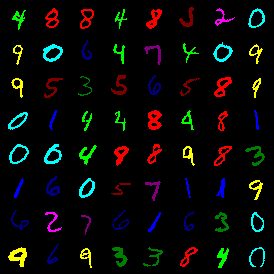
\includegraphics[width=\textwidth]{figures/cmnist-train.png}
    \caption{Training set: one-to-one mapping between colour and digit class.}%
    \label{fig:literature-cmnist-train}
  \end{subfigure}
  \quad\quad
  \begin{subfigure}[b]{0.4\textwidth}
    \centering
    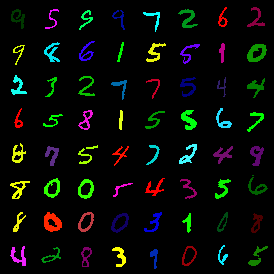
\includegraphics[width=\textwidth]{figures/cmnist-test.png}
    \caption{Test set: random assignment of colours.}%
    \label{fig:literature-cmnist-test}
  \end{subfigure}
  \caption{%
    A typical example of the Coloured MNIST dataset.
  }%
  \label{fig:literature-cmnist}
\end{figure}

\citet{kim2019learning} also consider the problem of learning from biased data (and evaluating on \emph{un}biased data).
While they do not formulate the problem as a fairness problem,
it is equivalent to enforcing fairness in the presence of severe sampling bias.
Their main motivating example is the Coloured MNIST dataset;
a dataset derived from the MNIST dataset~\citep{lecun1994mnist}.
In this dataset, digits are randomly coloured in the test set,
but in the training set there is a one-to-one correspondence between digit class and colour.
(See \figref{fig:literature-cmnist} for an example of this dataset.)
A na\"ive classifier will learn to predict colour instead of digit class.
The proposed method is very similar to \citet{ganin2016domain} and \citet{edwards2016censoring},
if we think of the colours as forming different domains
(\ie, the \emph{red} domain contains all red digits, etc.).
The goal is then to learn a domain-independent representation.
The main difference to previous work is an additional entropy loss term in the adversarial loss.

\citet{arjovsky2019invariant} tackle a similar problem, but take a very different approach,
which they term ``Invariant Risk Minimisation'', contrasted to the usual approach of \acf{ERM}.
As with \citet{kim2019learning},
the goal is to ignore spurious correlations that only appear in the very imperfect training set,
but not in the test set;
and they also perform experiments on Coloured MNIST.
They formalise the problem as one of different environments $e\in E$,
where each environment is a different, biased view of the same underlying data distribution.
The idea is to train a predictor that is simultaneously optimal for all the environments,
with the expectation that this generalises to the test set.
This idea is formulated as a (intractable) bi-level, constrained optimisation problem,
which they approximate with a tractable regularised optimisation.

As the authors point out,
the goal of machine learning should be to identify natural, deep, robust structures in reality,
instead of relying on superficial correlations.
(This dichotomy is sometimes framed as \emph{correlation} vs \emph{causality},
where ``causality'' takes on a very broad meaning that encompasses any kind of fundamental structure in reality; see also the discussion of \emph{causality} in \chapref{ch:introduction}.)
Under this view, methods for invariance learning can be framed as trying to learn a more fundamental structure
than the dataset at first seems to show.
By aiming to be invariant to specific environments/subgroups/domains (denoted by the variable \(s\)),
they can be seen as making the claim that \(s\) does not represent a natural structure,
but is merely an artefact of the data generation process.
Furthermore, the ground-truth-centric view of dataset bias can be understood as
aiming to identify the fundamental structures and aiming to be invariant to everything else.
This also fits with \citet{kim2019learning}'s work on Coloured MNIST:
colour is not regarded as the fundamental structure in the data.

\citet{creager2020environment} build directly on \citet{arjovsky2019invariant}.
They aim to address the limitation that the environments -- that one wants to be invariant to -- have to be pre-defined.
Their contribution is to infer these environments instead,
based on identifying which environment splits would most negatively affect an \ac{ERM} classifier.
Their experiments show that this can even improve upon human-designated environments;
experiments are performed on a synthetic dataset and Coloured MNIST.
In contrast to \citet{kim2019learning} and \citet{arjovsky2019invariant},
the authors explicitly point out the connection to traditional fairness methods.

A conceptually very influential work was \citet{friedler2016possibility}.
While this work does not explicitly present a ground-truth-centric approach to bias,
their concepts of the ``construct space'' and the ``observed space'' are close
to the idea of the (biased) training distribution and the true underlying distribution.

\citet{jiang2020identifying} also formulate their problem this way:
in their setting, the underlying unbiased labels become corrupted by a biased labeller,
which results in a biased training set.
Their goal is to train a classifier that makes correct predictions consistent with the true labels.
However, they treat the true labels as completely unknown
and evaluate their models w.r.t.\ the common fairness definitions on a test set
that is just as biased as the training set.

\citet{kallus2018residual} is another more conceptual work.
They present an intuitive model for how sampling bias can enter a training set
and how it can be very hard to correct for such a bias.
The paper refers to the process as \emph{systematic censoring},
but this is not meant to necessarily imply that this censoring was a conscious decision by some authority;
it can also be an unintended side effect of an enacted policy.
\emph{Systematic censoring} can arise any time a screening process prevents observing the outcome for the screened-out samples.
For example, if, historically, a certain demographic group was screened out from receiving loans,
then it was not possible to observe default rates for this group;
and so any historical data on defaulting is useless for that demographic group.
Even if a bank wants to change their policy,
it is hard to correct for the bias in the training set because there is no good data to learn from.
This is a prime example of a ground-truth-centric bias problem,
as defined in the beginning of the chapter.

Finally, as mentioned in the beginning,
\citet{blum2020recovering} provide a formalisation of a setting with label bias and sampling bias
and an unbiased ground-truth test set.
They explicitly state not being affected by a fairness-accuracy trade-off,
because the true distribution in the considered problem satisfies \acf{DP}.
Their formalised dataset generation process has multiple steps:
First, a small amount of random noise is applied to the (true) labels;
this models general inaccuracies in the labelling process and does not introduce bias yet.
Second, sampling bias is added, by dropping samples based on what the sample's \(s\) and \(y\) values are.
Concretely, only samples with \(s=0\) are dropped.
Finally, labelling bias is added, by flipping labels for one of the demographic groups (\eg, \(s=0\)),
in one specific direction (from \(y=1\) to \(y=0\)).
The authors show that in this specific situation,
an unbiased classifier (as determined by evaluation on the unbiased test set) can be recovered
by enforcing its predictions to be compatible with \acf{EOpp} on the training set.
Notably, the fairness constraint enforced during training (\ac{EOpp})
is not the fairness constraint satisfied by the predictions on the unbiased test set (\ac{DP}).
One reason, why enforcing \ac{EOpp} works so well here is
that the label bias only affects the \emph{underrepresented} demographic group,
and that the label bias is the direction (\(y=1\) to \(y=0\)) that \ac{EOpp} is most sensitive to.
Thus, even in the ground-truth-centric view of bias,
fairness constraints can be very useful.

\citet{maity2020notradeoff} provide a similar analysis to \citet{blum2020recovering},
but consider more general dataset biases.
Just like \citet{blum2020recovering}, they explicitly reject a fairness-accuracy trade-off,
because they evaluate on a balanced test set.
(In the paper this is formulated in terms of the optimal Bayes classifier satisfying their notions of fairness on the test set.)
They show that the sampling bias (in the training set) that they consider,
can be overcome by enforcing an appropriately chosen risk-based notion of algorithmic fairness;
either a notion they term \emph{risk parity} (inspired by \ac{DP})
or \emph{conditional risk parity} (inspired by \ac{EOdds}).

A perceived shortcoming of most methods in this area is that they rely on annotations for the subgroups.
Two papers that tried to circumvent this problem are \citet{HasSriNamLia18,nam2020learning},
both taking very different routes.
The first one tries to be robust with respect to all possible subgroups down to a certain size.
Essentially, the method tackles the worst-case scenario where the most egregiously misclassified samples form a subgroup.
The second approach is based on the idea that subgroups are easier to predict than the actual prediction targets.
After all, if this were not the case, then there would not really be a problem.
Thus, a classifier is learned in such a way that it predominantly tries to make ``easy'' predictions,
that is, samples where the model is very confident receive a higher weight.
The assumption is that this model learns to predict the subgroup (or spurious attribute),
for which no labels are available.
A second model is then trained, such that those samples are downweighted for which the first model was very confident;
the hope being that by learning the ``hard'' samples, the model learns the correct relationship.
Both \citet{HasSriNamLia18,nam2020learning} frame their methods as improving accuracy on an unbiased test set
and do not make references to fairness metrics,
but a strong connection to the fairness literature nevertheless exists.

% \section{Recent developments in Fairness}\label{recent-developments-in-fairness}
% At this point, fairness in machine learning has come a long way.
% There are several working implementations for various fairness criteria
% that give reasonable performance.
% Nevertheless, there are still many unexplored areas.

% There is, for example, a lot of other recent work on fair representation
% with adversarial neural networks.
% These approaches vary in the structure of the network and the objective function.
% These works are, however, all right now only in pre-print.
% There is \citet{edwards2016censoring}, \citet{beutel2017data}
% and \citet{zhang2018mitigating} for learning fair representations with adversaries.
% \citet{calmon2017optimized} improve on the work by \citet{zemel2013learning}.

% \citet{kilbertus2018blind} recently proposed a mechanism
% where the sensitive attributes are encrypted to avoid being used for discrimination.
% \citet{bechavod2017penalizing} use (as some others before) a regularisation approach to train fair classifiers.

% Finally, \citet{everitt2017reinforcement} investigate
% a problem in reinforcement learning that is similar to bias in classification.
% In the previously discussed papers,
% the bias originates from the training inputs or the training labels.
% In the work by \citet{everitt2017reinforcement},
% they consider the case of reinforcement learning (RL) with a corrupt reward signal.
% In this case, the RL algorithm might know that the reward is not correct,
% but does not know in what specific way it is not correct.
% The paper discusses some strategies to deal with this,
% but there are very many open questions.
